
\newpage

\section{Planner}

This section describes the planner algorithm implemented in the project.
\newline

Suppose we have access to a system whose behaviour must be controlled. 
This system must follow a sequence of trajectories, trajectories that define a sequence of target positions
the system will have to reach.
As it is possible for the system to reach these positions, it is also possible that it does not. 
Some external perturbations may affect the system, that would not reach its target positions.
Considering those perturbations forces to generate a target position knowing the system's current position.
The system will be said to be controlled in closed loop.

Theoretically, any point of any trajectory is a potential target.
The only pieces of informations we have to decide which point to choose are : 

\begint{itemize}

\item[-] the current position of the system; this information gives a way to compare two candidate target
points. Their positions relatively to the current position will help to decide which one to choose. 

\item[-] the previous target point, or the start position; this information gives a position to start 
searching for a target point; 

\end{itemize}

That being said, the generation of a target positon appears \footnote{and obviously is} a complex process.

A particular algorithm, called a planner, will be used for this purpose.

A planner is an algorithm that, given a sequence of trajectories, a point of a trajectory to start searching 
at, and a current position, searches the trajectories sequence from the start point for a valid target
position.

newline

In order to describe its main objectives more accurately, we need to elaborate a bit on the notion of 
trajectory.
\newline

\subsection{Trajectory}

Definition : a trajectory t is a continuous application from a segment of R in $R^n$ :
\newline

$t : [a, b] -> R^n$, $a$ and $b$ two real numbers, $n$ a positive integer, t continuous.
\newline

Naming convention : 
\begin{itemize}
\item [-] n : the dimension of the trajectory;
\item [-] x in [a, b] : an index of the trajectory;
\item [-] t(x), x in [a, b] : a point of the trajectory;
\item [-] a : the minimal index, the initial index;
\item [-] t(a) : the initial point;
\item [-] b : the maximal index, the final index;
\item [-] t(b) : the final point;
\newline
\end{itemize}

A trajectory $t$ represents a path in a particular space from its initial point $t_i$ to its final point 
$t_f$.

Its aim is to fully determine the path that some system must follow in this space;


\subsection{Target point choice}

As we stated earlier, any point of any trajectory is a candidate target, and the planner has to choose 
between all those possible points.
To do this, the planner considers the distance between a candidate target, and the current position.

The planner is given a positive interval, called the target interval, with the objective to
find a point of a trajectory whose distance from the current position belongs to the target interval.

Given the current position, the target interval defines a set of valid points, that verify the distance 
condition. 

The sequence of trajectories may or may not intersect this set in several portions of trajectories.

The planner must at first determine these candidate portions. Several parameters may influence the 
search. Among these parameters, is or is not the start position, that gives a point in the trajectory to start
searching at. 

When the planner has finished searching for candidate portions, it must choose a point in one of them. 
Many parameters may influence the choice. If trajectories must be followed in order, the planner may choose
the closest portion of trajectory to start point, and choose a point close to a distance target. 

If trajectories may be skipped, at the benefit of the traversal speed, the planner may choose the last 
candidate portion (closest to the end of the sequence), and also, choose a point close to a distance target.


\subsection{Hook mode}

No constraint has been imposed on trajectories in the trajectory sequence, except that trajectories must be 
continuous. Successive trajectories may be disjoint, ie, have separate initial and final points.

When reaching the final position of a trajectory, and attempting to reach the initial point of the next
trajectory, if the distance between stated points does not belong to the target interval, no valid target
point may be found.




%TODO REWRITE THIS
Let us consider now, two trajectories, $u$ and $v$ that share the same dimension, and must be followed one 
after the other, $u_i$, $u_f$, $v_i$, $v_f$ initial and final points of $u$ and $v$.
If both trajectories are joint, ie $u_f = v_i$, the path between $u_i$ and $v_f$ is fully determined.
If trajectories are disjoint, the path is simply undetermined, as there is no trajectory defined between
$u_f$ and $ v_i$to do so.
\newline

A planner can accept only a sequence of consecutively joint trajectories, or can accept any sequence of 
trajectories.
In the second case, it must contain a hook algorithm, that is in charge of determining an arbitrary path
from $u_f$ to $ v_i$.
The planer has to work modes, trajectory mode, where it processes a trajectory, and hook mode, where it 
attempts to reach a trajectory's initial point;

\newpage


\subsection{Transition point}

A transition point is a point where a brutal change of direction occurs.
\newline

As a planer can be used to control physical systems, that may suffer of this kind of changes, it may be 
important to monitor the existence of those points.
A planner can offer this monitoring, so that actions can be taken by another piece of code.
\newline

The presence of transition points inside trajectories is uncertain, and must be determined manually;
A planner can also offer this functionality, but it involves traversing the trajectory entirely, and 
it can be heavy for some low-performance systems;
\newline

However if we cannot easily detect transition points inside a trajectory, there are two immediate 
transition points, at extremal indices.
\newline

When completing a trajectory (reaching its final point), the planner may, enter into hook mode.
The hook algorithm is used to determine a path to the next trajectory's initial point.
This is the first transition point, as the direction the planner takes may not be the direction at the end
of the trajectory;
\newline

When the hook algorithm manages to reach the next trajectory's initial point, the planner goes into 
trajectory mode, and starts searching the trajectory for an adequate point.
This is the second transition point, as the direction the next trajectory takes may not be the direction 
the planner took to reach its initial point.
\newline


\subsection{Managing transition points}

The planner maintains a list referencing transition points in their order of appearance in the global 
path;
\newline

This list verifies the following conditions :
\begin{itemize}

\item[-] when the planner has processed all trajectories, the list is empty;

\item[-] when the planner is processing a trajectory, the first transition point in the list corresponds to 
the currenttrajectory's final point;

\item[-] when the planner is hooking the next trajectory, the first transition point in the list corresponds
to the initial point of the trajectory to hook;

\end{itemize}

This list is updated the following way :

\begin{itemize}

\item[-] When adding a trajectory to the planner's list, the planner determines if the trajectory is joint to 
its predecessor.
If so, it modifies the last transition point, to reflect the direction change due to the trajectory, 
and marks the transition to trigger trajectory mode.
If not, it modifies the last transition point, to reflect the direction change due to the hook algorithm, 
and mark it to trigger hook mode;
it then adds a transition point to monitor, at the initial point of the new trajectory, to reflect the 
direction change between the hook aglorithm and the trajectory;
Then, it attempts to find transition points in the trajectory.
If it finds some, it adds them in their order of appearance;
As stated earlier, this operation is time-consuming, and can be skipped.
Finally, it creates another transition point to monitor, representing the stop at the end of the new 
trajectory. This transition will be modified, when a new trajectory will be added, as described just before, 
to reflect a direction change instead of a stop.

\item[-] When processing a trajectory, when a transition point is reached inside the trajectory, the planner 
removes the first transition point of the list;

\item[-] At trajectory mode exit, when the planner reaches the last point of a trajectory, or at hook mode 
exit, when the planner has hooked the first point of a trajectory, it removes the first transition point, 
and depending on its type, it enters into hook mode, or trajectory mode;

\end{itemize}

\newpage

\subsection{Trajectory mode}

Following a trajectory is a primary objective for a control system. It is the base objective.
The planner's objective is to decide of a target position. After this decision, multiple corrections
or error sources, or perturbations may intervein, that the planner will not be aware of. 
This will result in a final position that may not be the one the planner previously picked. 
Because of this, to choose a target point, the planner must take the current known position into account.
\newline 

The planner will comprise an algorithm whose purpose is, given a position $P$ (that may not belong to 
the trajectory),to select a point of the trajectory that verifies a distance condition.
For example, the planner may have to pick a point of the trajectory whose maximal or minimal or average 
distance from the provided position is within a certain range $[d_{min}, d_{max}]$.
\newline

More verbosely, the planner disposes of a distance function $d : R^n \times R^n \rightarrow R^+$, 
that takes two points in arguments, and returns a real number, that we will call the distance.
It also posseses a target interval $I = [d_{min}, d_{max}]$ , and a distance target $d_{target}$, that verify
 $d_{min} < d_{target} < d_{max}$.
The planner's goal will be to find a point $Q$, as $d(P, Q) \in I$, as close as $d_{target}$ as possible.
\newline

Given $t$ a trajectory to process, $P$ the position, $d$ the distance function, we can define $D$ the reduced
 distance function :
$D : R \rightarrow R^+, i -> d(P, t(i))$ 
that gives the distance from the position of the point of $t$ at index i.
This function will indicate the planner if a point is close enough to the current position to be considered
as already visited. 
\newline

The objective of the planner is, given a position $P$, a trajectory $t$, a distance function $d$, 
a probable index $i_e$ (e for estimate), and a probable index delta $\delta _i$ to determine, in a minimal 
number of computations, an index $i_f$ (f for final) as $f(i_v)) \in [d_{min}, d_{max}]$.
$i_e$ and $\delta _i$ are two important parameters. The first will determine the first index whose distance
should be computed. If its distance is not in the target interval, $\delta _i$ will be used, to determine the
next point to be evaluated. 
\newline 

This problem as it is a classical analysis problem, and can be solved with many methods;
Though, an aditional rule comes to complexify the resolution. 
Indeed, as the planner's goal is to traverse the whole trajectory, it should prioritise points with high
indices. A simpler rule that is not equivalent but easier to work with, is that the cost should increase 
when increasing the index, at the choosen point.
\newline

A fact to remember, is that the index where the search begins is purely speculative. In case of inacurate 
prediction, different cases can occur.

\newpage

\subsection{Prediction}

We develop here the first stage of the determination of a point. Depending on the exactitude of $i_e$, several
cases are encountered.

\begin{figure}[!h]
\fbox{\centerline{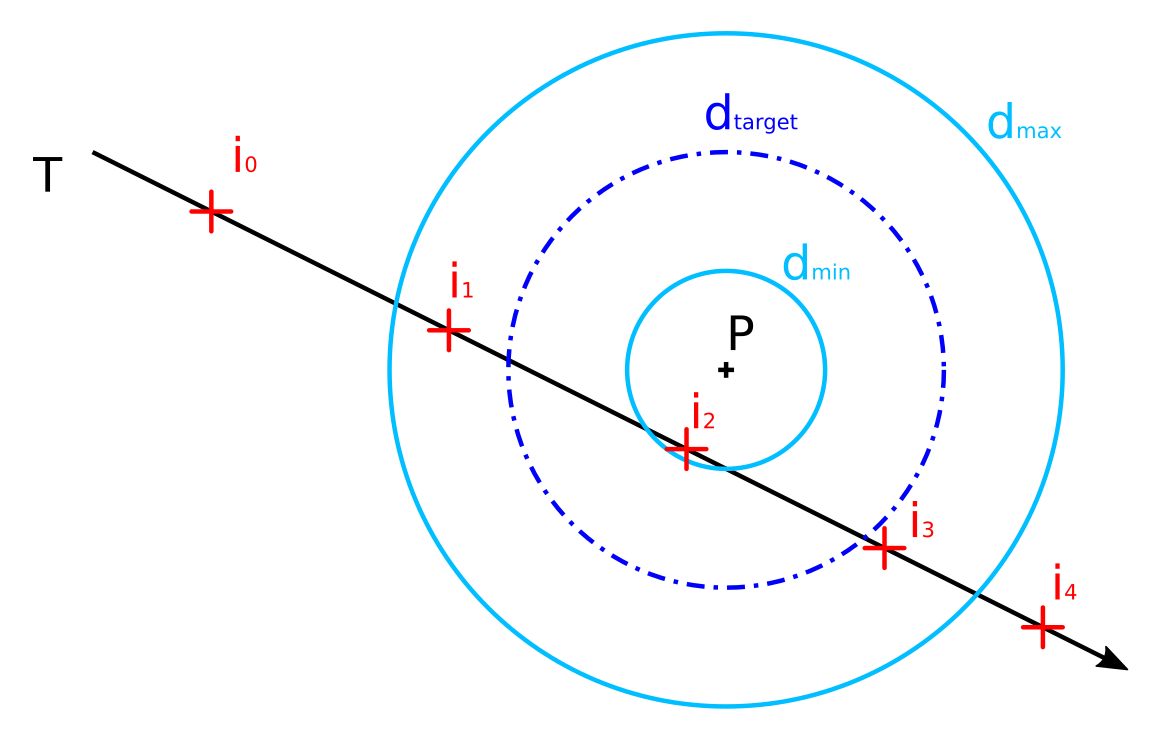
\includegraphics[width=12cm]{sections/traj_cases.png}}}
\caption{Different cases, depending on the index prediction}
\end{figure}

The figure behind shows different cases that may occur, for different values of $i_e$, with a simple example :
the trajectory $T$ to follow is a simple 2D line, and the distance considered is the geometric distance.
$P$ the current position, and circles delimitating the acceptable positions set are drawn accordingly.

Different cases are : 
\begin{itemize}

\item [-] $i_0$, critical traction : $i_e$ is highly underestimated, the distance to the posion being
superior to the maximal bound, incrementing the index making this distance decrease. In this situation, simply
increasing the index until a valid one is found is not enough, because it would lead to choose a point where
the previously enounced rule doesn't apply. In this case, the planner must increase the index, until the 
distance starts increasing and consider points beyond that index only.

\item [-] $i_1$, ghost traction : same case as before, but this time, the estimation gives a valid distance. 
This case is a little bit problematic, as the estimation seems to be valid, but is a matter of fact, 
counterveins to our decision rule. In this case again, the index must be increased until the distance 
increases, and only consider points beyond that index.

\item [-] $_i2$, traction : the prediction lead to a point too close to the current position. This point is 
already visited, and can't be selected. Once again, the index must be increased until the distance increases
, and only indices beyond must be considered during the search.

\item [-] $i_3$, correct prediction : the prediction lead to an acceptable point.

\item [-] $i_4$, resistance : $i_e$ is overestimated, the distance to the position being superior to the
maximal bound, incrementing the index making this distance increase. A suitable point must be seatched before
the estimated index.

\end{itemize}

\newpage

\subsection{Search procedures}

In the list behind, two procedures were implicitely refered : 
\begin{itemize}

\item[-] the slide. Given two indices and their associated distances, the trajectory is traversed in the 
local descending direction, until a local minimum is found, or until the distance decreases 
over a certain target value, or the slide arrives to an extremal index;

\item[-] the raise. Given two points, and their associated distances, the trajectory is traversed in the
local descending direction, until a point at a sufficient distance is found, or the raise reach an extremal 
index;

\item[-] the windowing. Given two points, and their associated distances $d_0$ and $d_1$, 
the trajectory is traversed until a point at a position belonging to an interval 
$D \in [d_0, d_1]$ is found.

\end{itemize}


\subsection{Algorithm}












At the beginning stage of the algorithm, only the point at $i_e$ and its distance are computed.
No indication is available on how the distance will vary when the index does. 
As you may have seen, this information alone does not suffice to determine in which case 
we are.
We can only determine that we are in $i_1$ or $i_3$, or that we are in $i_2$, or that we are 
in $i_0$ or $i_4$.
To go further, a second point will be determined, its index being given by $\delta _i$, and different actions
will be taken.
\newline

Different cases are : 

\begin{itemize}

\item[-] $i_1$ or $i_3$ : within the acceptable bounds : 
the second point is used to determine the current case.
If the distance increases when the index increases (positive derivative), we are in case 
$i_3$ and the point is acceptable. 
If not, we are in case $i_1$, and a slide must be executed.
At the local minimal point, we are either in case $i_3$, which gives us an acceptable point, or in case $i_2$.

\item[-] $i_2$ : below the minimal distance : the estimated point is considered as already visited. 
A raise must be executed, to the minimal distance.
If a point below the maximal distance is found, we are in $i_3$, which gives us an acceptable point.
If a point beyond the maximal distance is found, the windowing gives us an acceptable point.
If no point is found, the trajectory is finished.

\item[-] $i_0$ or $i_4$ : beyond the maximal distance :
the second point is used to determine the current case.  
If the distances increases with the index increasing, we can suppose we are in $i_4$. If not, we are in $i_1$.
A slide is executed, targetting the maximal value, if we are in $i_1$. If in $i_4$, we need to 
reach the minimum.
Here comes a problem : there is no guarantee that the local minimum is in the distance bounds, as the
direction to take is extrapolated from evaluated points, which has no guarantee to be accurate. 
There is either no guarantee that a point in the distance bounds exists, as the current position could be too
far from the trajetory.
If we are in $i_4$, if a local minimum was detected, and the maximal distance has never been reached, 
the planner has failed to compute the point. If the maximal distance has been reached, we either 
have determined a valid point, or can use the windowing to compute one.
If we are in $i_1$, and the local minimum is not lower than the maxmal distance, the planner has failed to 
compute the point. If not, we end up in $i_3$, which gives us a valid point, or in $i_2$, which leads us to 
a valid point.

\end{itemize}

\newpage

\subsection{Limit cases}




\subsection{Faults}

\subsection{Interrupt levels}


